\makeatletter\def\input@path{{styles/}{corps/}{bib/}}\makeatother

\documentclass{transp_java}

\title[Introduction � l'algorithmique]{Introduction � l'algorithmique}
\author{Rod�ric Moiti�}
%\date[DLT 2003]{Developments in Language Theory Conference, 2003}
\date{}
\institute{ENSIETA}

\usepackage{aeguill}
\usefonttheme{professionalfonts} 

\def\mcT{\ensuremath{\mathcal T}}
\def\mcF{\ensuremath{\mathcal F}}
\usetikzlibrary{automata}

%\usetheme{Transp}
\usetheme{progressbar}
%\usetheme{Darmstadt}
%\definecolor{progressbar@bgblue}{rgb}{0.95,0.75,0.75} % use structure theme to change
%\definecolor{progressbar@fgblue}{rgb}{0.9,0.1,0.1} % use structure theme to change
\progressbaroptions{imagename=java_logo2.png}

\mode<handout>{
  \usecolortheme{dove}
  \usepackage{pgfpages}
  \pgfpagesuselayout{4 on 1}[a4paper, border shrink=5mm, landscape]
}



\begin{document}

\frame{\titlepage}

\AtBeginSection[]
{
  \begin{frame}<beamer>
    \frametitle{Sommaire}
    \tableofcontents[current,currentsection]
  \end{frame}
}

\AtBeginSubsection[]
{
  \begin{frame}<beamer>
    \frametitle{Sommaire}
    \tableofcontents[current,currentsubsection]
  \end{frame}
}


%%%
\section{Calculs de complexit�}

\subsection{Notions sur la  complexit�}

\begin{frame}
  \frametitle{Complexit�s}
  \begin{definition}[Complexit� en temps]
    On appelle complexit� d'un algorithme le nombre d'op�rations
    �l�mentaires effectu�es par cet algorithme pour traiter un jeu de
    donn�es de taille $n$.
  \end{definition} \pause

  \begin{definition}[Complexit� dans le pire des cas]
    La complexit� dans le pire des cas d'un algorithme est la complexit� de
    cet algorithme pour le jeu de donn�es le plus d�favorable.
  \end{definition} \pause

  \begin{definition}[Complexit� moyenne]
    La complexit� moyenne d'un algorithme est la moyenne des complexit�s pour
    tous les jeux de donn�es possibles.
  \end{definition}
\end{frame}


\begin{frame}
  \frametitle{Complexit�s}

  \textbf{Complexit� en temps}

    \begin{itemize}[<+->]
    \item Donald Knuth fut un des premiers � l'appliquer ;
    \item �valuation de l'efficacit� des algorithmes ;
    \item nombre d'op�rations par rapport � la taille des entr�es ;
    \item �valuation dans le pire des cas, en moyenne.
    \end{itemize}

    \pause
    \textbf{Complexit� en espace}
    \begin{itemize}
    \item mesure de l'espace m�moire utilis�
    \end{itemize}
\end{frame}


\begin{frame}
  \frametitle{Exemple : recherche d'un �l�ment}
  Entr�e~: ensemble ordonn� d'entiers $E = \left\{x_1, x_2, \ldots,
    x_n\right\}$ \emph{i.e.}
  $x_1 \leqslant x_2 \leqslant \ldots \leqslant x_n$
  \vspace{5mm}
  \pause
  {\small
\begin{procedure}[H]
  \caption{Recherche(Ensemble $E$, entier n)}
  \KwData{i : entier}
  \For{$i \in [1,n]$} {
    \If{$x_i = y$ \tcp{Op�ration �l�mentaire}} {
      exit \;
    }
  }
\end{procedure}
  %   \begin{algorithmic}[1]
  %     \Procedure{recherche}{Ensemble $E$, entier $y$}
  %       \Var
  %         \State i : entier
  %       \EndVar
  %       \For{$i \in [1,n]$}
  %         \If{$x_i = y$} \Comment op�ration �l�mentaire
  %           \State exit
  %         \EndIf
  %       \EndFor
  %   \EndProcedure
  % \end{algorithmic}
}
\end{frame}

\begin{frame}
  \frametitle{Exemple : complexit� dans le pire des cas}

  \begin{block}{Identifier le pire des cas}
    \uncover<2->{
      Dernier �l�ment de l'ensemble
    }
  \end{block}

  \uncover<3->{
  \begin{block}{Calculer avec ce jeu de donn�es}
    \begin{itemize}
    \item<4-> $C(n) = n$ 
    \end{itemize}
  \end{block}
  }
\end{frame}

\begin{frame}
  \frametitle{Exemple : complexit� moyenne}

  \begin{block}{Inventaire des situations possibles}
    \begin{itemize}
    \item<2-> \emph{y} en premi�re position
    \item<3-> \emph{y} en deuxi�me position
    \item<4-> \ldots
    \end{itemize}
  \end{block}

  \uncover<5->{
  \begin{block}{Calculer la moyenne}
    \begin{itemize}
    \item<6-> $n$ jeux de donn�es
    \item<7-> $\displaystyle C(n) = \frac{1}{n} \left(1 + 2 + \ldots + n\right)$ 
    \item<8-> $\displaystyle C(n) = \frac{1}{n} \frac{n(n+1)}{2}$ 
    \item<9-> $\displaystyle C(n) = \frac{n+1}{2}$ 
    \end{itemize}
  \end{block}
  }
\end{frame}



\begin{frame}
  \frametitle{Exemple : recherche d'un �l�ment par dichotomie}
  {\small
\begin{procedure}[H]
  \caption{Recherche(Ensemble $E$, entier n)}
  \KwData{i, min, max : entier}
  $min \gets 1$, $max \gets n$ \;
  \While{$min \leqslant max$} {
    $i \gets (max+min)/2$ \;
    \uIf{$x_i = y$ \tcp{Op�ration �l�mentaire}} {
      exit \;
    }
    \uElseIf{$y < x_i$} {
      $max \gets i-1$ \;
    }
    \Else {
      $min \gets i+1$ \;
    }
  }
\end{procedure}
  %   \begin{algorithmic}[1]
  %     \Procedure{recherche}{Ensemble $E$, entier $y$}
  %       \Var
  %         \State min, max, i : entier
  %       \EndVar
  %       \State $min \gets 1$, $max \gets n$
  %       \While{$min \leqslant max$}
  %         \State $i \gets (max+min)/2$
  %         \If{$y = x_i$} \Comment op�ration �l�mentaire
  %           \State exit
  %         \ElsIf{$y < x_i$}
  %           \State $max \gets i-1$
  %         \Else
  %           \State $min \gets i+1$
  %         \EndIf
  %       \EndWhile
  %   \EndProcedure
  % \end{algorithmic}
}
\end{frame}

\begin{frame}
  \frametitle{Exemple : complexit� dans le pire des cas}

  \begin{block}{Identifier le pire des cas}
    \uncover<2->{
      Premier ou dernier �l�ment de l'ensemble
    }
  \end{block}

  \uncover<3->{
  \begin{block}{Calculer avec ce jeu de donn�es}
    \begin{itemize}
    \item<4-> $C(1) = 1$
    \item<5-> $C(n) = 1 + C(n/2)$
    \item<6-> Soit $k = \lceil \log_2 n\rceil$
    \item<7-> $C(2^k) = 1 + C(2^{k-1})$
    \item<8-> $C(n) = C(2^k) = k+1 = \lceil \log n\rceil + 1$
    \end{itemize}
  \end{block}
  }
\end{frame}

\begin{frame}
  \frametitle{Exemple : complexit� moyenne}
  \begin{alertblock}{Calcul de la complexit� moyenne}
    Complexit� moyenne\\

    \uncover<2>{\ldots{} laiss�e � titre d'exercice}
  \end{alertblock}
\end{frame}




\begin{frame}
  \frametitle{Exemple : recherche d'un �l�ment}
  \begin{itemize}
  \item entr�e : ensemble d'entiers $x_1, x_2, \ldots, x_n$
  \item nombre d'op�rations :
    \begin{itemize}
    \item $\displaystyle\frac{n+1}{2}$
    \item $\lceil \log n\rceil + 1$
    \end{itemize}
  \end{itemize}\pause
  \begin{itemize}
  \item formules lourdes � manipuler
    \pause
  \item solution : notation de Landau
  \end{itemize}
\end{frame}

\subsection{Notation de Landau}

\begin{frame}
  \frametitle{Ordres de grandeur}
  Seul le terme dominant est utilis�

  Exemple : 
  $an^2+bn+c\log n +d$\only<2->{$\leadsto an^2$}\only<3->{$\leadsto n^2$}

  \uncover<4->{
  Notation $\Theta, O, \Omega$ :
  \begin{eqnarray*}
    \uncover<4->{\Theta(g(n)) =} &\uncover<4->{\{f(n) : \exists c_1,c_2\in
      \nbR^+, n_0\in\nbN / \forall n\geqslant n_0 , }\\ 
    &\uncover<4->{0 \leqslant c_1g(n) \leqslant f(n) \leqslant c_2g(n)\}}\\ 
    \uncover<5->{O(g(n)) = }&\uncover<5->{\{f(n) : \exists c\in \nbR^+,
      n_0\in\nbN / \forall n\geqslant n_0 ,} \\ 
    &\uncover<5->{0 \leqslant f(n) \leqslant cg(n)\}}\\ 
    \uncover<6->{\Omega(g(n)) = }&\uncover<6->{\{f(n) : \exists c\in \nbR^+,
      n_0\in\nbN / \forall n\geqslant n_0 ,} \\
    &\uncover<6->{0 \leqslant cg(n) \leqslant f(n) \}}
\end{eqnarray*}  
}
\end{frame}


\begin{frame}
  \frametitle{Bons algorithmes}
\centering\begin{tabular}{|l||l|l|l|l|l|}
\hline
 & 20 & 50 & 100 & 200 & 500 \\
\hline
\hline
$10^3n$ & 0.02 s & 0.05 s & 0.1 s & 0.2 s & 0.5 s\\
\hline
$10^3n\log n$ & 0.09 s & 0.3 s & 0.6 s & 1.5 s & 4.5 s \\
\hline
$100n^2$ & 0.04 s & 0.25 s & 1 s & 4 s & 25 s  \\
\hline
$10n^3$ & 0.02 s & 1 s & 10 s & 1 mn & 21 mn \\
\hline
$n^{\log n}$ & 0.4 s & 1.1 h & 220 j & 12500 ans & $5.10^{10}$ ans  \\
\hline
$2^\frac n3$ & $10^{-4}$ s & 0.1 s & 2.7 h & $3.10^6$ ans &  \\
\hline
$2^n$ & 1 s & 36 ans& & &  \\
\hline
$3^n$ & 58 mn & $2.10^{11}$ ans & & & \\
\hline
$n!$ & 77100 ans & & & & \\
\hline
\end{tabular}

\end{frame}

\section{Classes de complexit�}

\subsection{Machine de Turing}

\begin{frame}
  \frametitle{Machines de Turing}
  \begin{itemize}
  \item D�crites en 1936 par Alan Turing
  \item Mod�le d'ordinateur
  \item Composition~:
    \begin{itemize}
    \item bande infinie des deux c�t�s (m�moire)
    \item t�te de lecture
    \item un �tat interne
    \item une fonction de transition
    \end{itemize}
  \end{itemize}
\end{frame}

\begin{frame}
  \frametitle{Notations}

  \begin{itemize}
  \item $\mcF_\star$ : ensemble des fonctions $f: \nbN^k \Rightarrow \nbN$
  \item On note~: $\lambda x_1\ldots x_n[f(x_1,\ldots,x_n)]$
  \item $k$~: arit� de $f$
  \item $\mcF_k$ fonctions de $\mcF_\star$ d'arit� $k$
  \item $\displaystyle\mcF_\star = \bigcup_{k\in\nbN}\mcF_k$
  \end{itemize}
\end{frame}


\begin{frame}
 \frametitle{D�finition formelle d'une machine de Turing}  
 $\mcT=\{ Q, A, \square, \delta, q_0\}$
 \begin{itemize}[<+->]
 \item $Q$ ensemble fini d'�tats
 \item $A$ ensemble fini de symboles (alphabet)
 \item $\square$ symbole blanc
 \item $\delta: Q\times A\cup\{\square\} \rightarrow \left(A\cup\{\square\}\right) \times
   \{L,R,N\} \times Q$ une
   fonction de transition (L=left, R=right, N=none)
 \item $q_0 \in Q$ l'�tat initial
 \end{itemize}
 \uncover<6->{ Avec~: $Q$ et $A$ deux ensembles finis disjoints et $\square \not\in A\cup Q$\\}
 \uncover<7->{On note $\hat{A} = A \cup \{\square\}$}
\end{frame}

\begin{frame}
  \frametitle{Exemple}

  \begin{exemple}
    Machine de Turing $\mcT$ calculant $\lambda x[2x]$\\
    Id�e~:
    \begin{itemize}[<+->]
    \item Si on est sur un blanc $\Rightarrow$ accept
    \item Pour tous les 1 du nombre
      \begin{itemize}
      \item Effacer le premier 1
      \item Ajouter deux 1 en fin de nombre
      \end{itemize}
    \item � la fin, se placer sur le premier 1
    \item Pour que tout fonctionne, s�parer les 1 des deux nombres par $\square$
    \end{itemize}
  \end{exemple}
\end{frame}

\begin{frame}
  \frametitle{Exemple~: automate}
  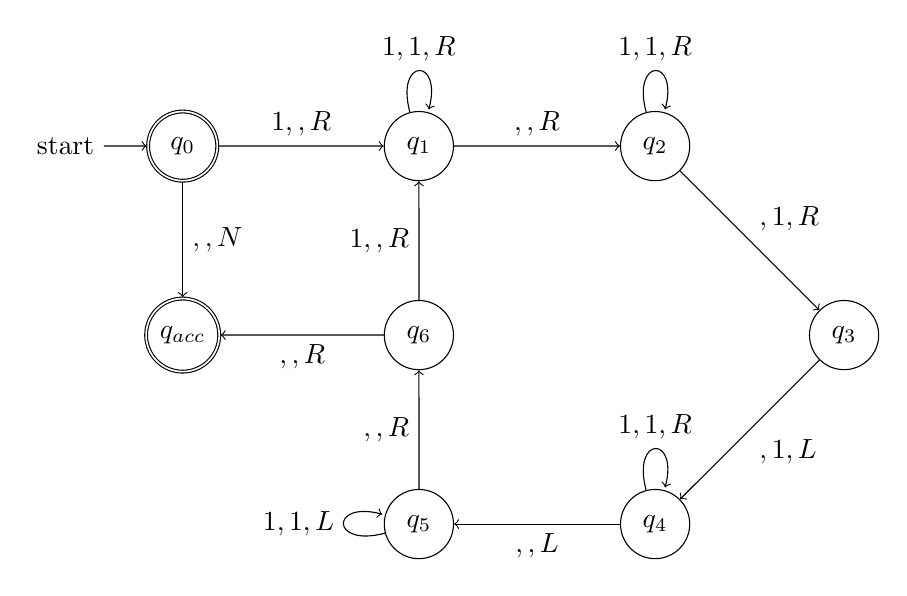
\begin{tikzpicture}[node distance=1cm,auto,scale=1.2]
    \node[state,initial,accepting] at (0,4) (q_0) {$q_0$};
    \node[state] at (2.5,4) (q_1) {$q_1$};
    \node[state] at (5,4) (q_2) {$q_2$};
    \node[state] at (7,2) (q_3) {$q_3$};
    \node[state] at (5,0) (q_4) {$q_4$};
    \node[state] at (2.5,0) (q_5) {$q_5$};
    \node[state] at (2.5,2) (q_6) {$q_6$};
    \node[state,accepting] at (0,2) (q_7) {$q_{acc}$};
    \path[->] (q_0) edge node {$1,\square,R$} (q_1)
              (q_1) edge node {$\square,\square,R$} (q_2)
              (q_2) edge node {$\square,1,R$} (q_3)
              (q_3) edge node {$\square,1,L$} (q_4)
              (q_4) edge node {$\square,\square,L$} (q_5)
              (q_5) edge node {$\square,\square,R$} (q_6)
              (q_6) edge node {$1,\square,R$} (q_1)
              (q_6) edge node {$\square,\square,R$} (q_7)
              (q_0) edge node {$\square,\square,N$} (q_7)
              (q_1) edge [loop above] node {$1,1,R$} ()
              (q_2) edge [loop above] node {$1,1,R$} ()
              (q_4) edge [loop above] node {$1,1,R$} ()
%              (q_4) edge [loop above] node {$1,1,L$} ()
              (q_5) edge [loop left] node {$1,1,L$} ()
              ;
  \end{tikzpicture}
\end{frame}

\begin{frame}
  \frametitle{Exemple~: table des transitions}

  Fonction $\delta$~:\\

  \begin{tabular}{|l|c|c|}
    \hline
    & $\square$ & 1 \\
    \hline
    $q_0$ & $\square, N, q_{acc}$  & $\square, R, q_1$ \\
    \hline
    $q_1$ & $\square, R, q_2$  & $1, R, q_1$ \\
    \hline
    $q_2$ & $1, R, q_3$  & $1, R, q_2$ \\
    \hline
    $q_3$ & $1, L, q_4$  & \\
    \hline
    $q_4$ & $\square, L, q_5$  & $1, L, q_4$ \\
    \hline
    $q_5$ & $\square, R, q_6$  & $1, L, q_5$ \\
    \hline
    $q_6$ & $\square, R, q_{acc}$  & $\square, R, q_1$ \\
    \hline
  \end{tabular}
\end{frame}

\begin{frame}
  \frametitle{Machine de Turing non d�terministe}
  Principe~:
  \begin{itemize}[<+->]
  \item remplacer $\delta$ par une partie de $Q \times \hat{A} \times \hat{A}
    \times \{R, L, N\} \times Q$
  \item[$\Rightarrow$] plusieurs choix de transition
  \item[$\Rightarrow$] ind�terminisme
  \end{itemize}
  \uncover<4->{
    Autre vision des choses~:
    \begin{itemize}
    \item<5-> Machine de Turing munie d'un oracle
    \item<6-> Principe~: v�rifier la solution fournie par l'oracle
    \end{itemize}
  }
\end{frame}

\subsection{Th�orie de la complexit�}

\begin{frame}
  \frametitle{Th�orie de la complexit�}
  \textbf{Objectif}~: d�terminer les probl�mes intrins�quement difficiles.\pause

  \begin{defi}[Probl�me d�cidable/ind�cidable]
    Un probl�me de d�cision est dit d�cidable s'il existe un algorithme (ou
    une machine de Turing) qui le d�cide. Sinon il est ind�cidable.
  \end{defi}\pause

  \begin{itemize}
  \item Probl�me ind�cidable : difficile
    \begin{itemize}
    \item Exemple : probl�me de l'arr�t
    \end{itemize}\pause
  \item Autre probl�mes difficiles ?
  \end{itemize}
\end{frame}

\begin{frame}
  \frametitle{Th�orie de la complexit�}
  \begin{itemize}
  \item donn�es en entr�e
  \item question sur ces donn�es
  \item r�ponse oui/non
  %\item extension aux probl�mes d'optimisation
  \end{itemize}\pause
  \begin{exemple}[Probl�me SAT]
    \only<-2>{
      \begin{itemize}
      \item $X=\{x_1, ..., x_n\}$ variables bool�ennes.
      \item $E=C_1 \wedge ... \wedge C_m $ expression
      \item $\forall i, C_i = u_{i1} \vee ... \vee u_{ik}$
      \item $u_{ij}$ : variable de $X$ compl�ment�e ou non
      \item Probl�me : d�terminer $x_i$ tel que $E=vrai$
      \end{itemize}}
    \only<3>{
      Ex~:\\
      $E=(x_1 \vee x_2 \vee \bar{x_3}) \wedge (\bar{x_1} \vee
      x_2) \wedge (x_3)$\\
      r�ponse \emph{VRAI} pour $x_1=0$ ou 1, $x_2 = 1$, $x_3 = 1$.
    }
  \end{exemple}
\end{frame}

\begin{frame}
  \frametitle{Classes P/NP}
  \begin{defi}[Classe P]
    ${\mathcal P} \in P $~: il existe un algorithme polynomial permettant de
    le r�soudre
  \end{defi}
  \pause
  \begin{exemple}[Classe P]
    \begin{itemize}
    \item Recherche d'un �l�ment dans un tableau
    \item Probl�mes de tris
    \end{itemize}
  \end{exemple}
  \pause
  Algorithme polynomial = � bon � algorithme
\end{frame}

\begin{frame}
  \frametitle{Classes P/NP}
  \begin{defi}[Classe NP]
    ${\mathcal P} \in NP $~: il existe un algorithme polynomial sur une
    machine de Turing non d�terministe permettant de le r�soudre
  \end{defi}
  \pause
  \begin{defi}[Classe NP]
    ${\mathcal P} \in NP $~: il existe un algorithme polynomial sur une
    machine de Turing d�terministe permettant de v�rifier une solution de
    $\mathcal P$.
  \end{defi}
\end{frame}

\begin{frame}
  \frametitle{Remarques classe NP}
\begin{itemize}[<+->]
\item $NP \neq$ probl�mes non polynomiaux
\item $NP=$ probl�mes v�rifiables en temps polynomial
\item $P \subseteq NP$
\item autre inclusion ?
\item probl�me � \$1.000.000
\end{itemize}
\end{frame}


\begin{frame}
  \frametitle{Classes}
  Quelques classes de complexit� :
  \begin{itemize}
  \item L/NL : algorithme logarithmique en espace
  \item P/NP/Co-NP : algorithme polynomial en temps
  \item PSPACE/NPSPACE : algorithme polynomial en espace
  \item EXPTIME : algorithme exponentiel en temps
  \end{itemize}
\end{frame}

\begin{frame}
  \frametitle{R�duction polynomiale}
  \begin{defi}[R�duction polynomiale]
    Un probl�me $\mathcal P_1$ se r�duit polynomialement � un probl�me
    $\mathcal P_2$ s'il existe un algorithme $\mathcal A_1$ r�solvant
    $\mathcal P_1$, faisant appel � un algorithme $\mathcal A_2$ r�solvant
    $\mathcal P_2$, et tel que si $\mathcal A_2$ est suppos� �l�mentaire,
    alors $\mathcal A_1$ est polynomial.
    On note $\mathcal P_1 \triangleright \mathcal P_2$.
  \end{defi}

  \begin{defi}[Probl�mes �quivalents]
    Deux probl�mes $\mathcal P_1$ et $\mathcal P_2$ sont dits polynomialement
    �quivalents si $\mathcal P_1 \triangleright \mathcal P_2$ et $\mathcal P_2
    \triangleright \mathcal P_1$. On note $\mathcal P_1 \bowtie
    \mathcal P_2$. 
  \end{defi}
\end{frame}

\begin{frame}
  \frametitle{Probl�mes NP-Complets}
  \begin{defi}[Probl�me NP-difficile]
    Un probl�me est NP-difficile si tout probl�me de NP se r�duit
    polynomialement � lui.
  \end{defi}\pause
  \begin{remarque}
    Un probl�me NP-difficile n'est pas forcement dans NP.
  \end{remarque}\pause
  \begin{defi}[Probl�me NP-complet]
    Un probl�me est NP-complet s'il est NP-difficile et qu'il est dans NP.
  \end{defi}
\end{frame}

\begin{frame}
  \frametitle{Th�or�me de Cook}
  \begin{theoreme}[Cook]
    Il existe des probl�mes NP-complets.
  \end{theoreme}\pause
  \begin{proof}
    Voir l'article � The Complexity of Theorem Proving Procedures � ref.
    � Proceedings of the third annual ACM symposium on Theory of
    computing, The Complexity of Theorem Proving Procedures, Stephen Cook,
    1971, pages = 151-158 �.
  \end{proof}
  \begin{itemize}
  \item beaucoup de probl�mes dans cette classe
  \item impossibilit� de les r�soudre efficacement (non d�terminisme)
  \end{itemize}
\end{frame}

\begin{frame}
  \frametitle{Probl�me 3-SAT}
  \begin{defi}[3-SAT]
    Le probl�me 3-SAT est un cas particulier du probl�me SAT lorsque la taille
    des clauses est exactement de 3.
  \end{defi}
  \begin{exemple}
    $E=(x_1 \vee x_2 \vee x_3) \wedge (\bar{x_1} \vee
    x_2 \vee x_4) \wedge (\bar{x_1} \vee x_2 \vee \bar{x_5}) \wedge (\bar{x_3}
    \vee x_4 \vee x_5)$
  \end{exemple}
  \begin{theoreme}
    3-SAT est NP-complet.
  \end{theoreme}
  \begin{proof}
    Preuve fournie par Richard M. Karp dans son article � In Complexity of
    Computer Computations � de 1972.
  \end{proof}
\end{frame}

\begin{frame}
  \frametitle{Probl�me du sac � dos}
  \begin{block}{Probl�me}
    Soit $S$ un ensemble fini d'entiers positifs. Soit $t \in \nbN^\star$.\\
    Probl�me~:
    \[\displaystyle\exists ? A \subset S / \sum_{x\in A} x = t
    \]
  \end{block}
  \pause
  \begin{theoreme}
    Le probl�me du sac � dos est NP-complet.
  \end{theoreme}
\end{frame}

\begin{frame}
  \frametitle{Preuve}
  Id�e~: construire une r�duction de 3-SAT vers le sac � dos.\\

  \begin{block}{Preuve}
    \begin{itemize}[<+->]
    \item Soit un ensemble de clauses $c_1,\ldots,c_m$ d'au plus 3 litt�raux.
    \item On num�rote les variables~: $q_1,\ldots,q_n$
    \item On pose~:
      \[
      \left\{\begin{array}{ll}
          k_i=8^{i-1} & i\in\{1,\ldots,n\}\\
          l_j=8^{n+j-1} & j\in\{1,\ldots,m\}
        \end{array}
      \right.
      \]
    \item Pour $i\in\{1,\ldots,n\}$, on d�finit~:
      \[
      \left\{\begin{array}{ll}
          n_i &= k_i + \sum\{l_j : q_i \mbox{ appara�t dans } c_j\}\\
          m_i &= k_i + \sum\{l_j : \bar{q_i} \mbox{ appara�t dans } c_j\}\\
        \end{array}
      \right.
      \]
  \end{itemize}
    \end{block}
\end{frame}

\begin{frame}
  \frametitle{Preuve (suite)}

  \begin{proof}[Preuve (suite)]
  $S$ contient~:
  \begin{itemize}
  \item les $n_i$et les $m_i$
  \item les $l_j$ et les $2l_j$
  \end{itemize}
  $t$ vaut~: $\displaystyle \sum_{i=1}^nk_i + 4\left(\sum_{j=1}^ml_j\right)$
  (en base 8~: $m$ 4 et $n$ 1).\\
  Cet algorithme est polynomial.
    
  \end{proof}
\end{frame}

\begin{frame}
  \frametitle{Justification de la preuve}
  \begin{itemize}
  \item Interpr�ter les nombres en base 8. Alors~:
    \begin{itemize}
    \item l'addition d'une partie de $S$ se fait sans retenue
    \item la somme d'une partie de S vaut $t$ si exactement 1 $n_i$, $m_i$ est
      dans la somme.
    \end{itemize}
  \item On d�finit $\tau_A(q_i) = 1 \Leftrightarrow n_i \in A$
  \item $\tau_A$ satisfait chaque $c_j$
    \begin{itemize}
    \item $(n+j)\ieme$ chiffre de $t$ vaut 4, donc il ne vient pas
      uniquement de $l_j$ et $2l_j$
    \end{itemize}
  \item Donc~: 
    \begin{itemize}
    \item $\exists n_i \in A$ tel que $u=q_i\in c_j$
  \item Ou~: $\exists m_i \in A$ tel que $u=\bar{q_i} \in c_j$
  \item Dans les 2 cas~: $\tau_A(u) = 1$
    \end{itemize}
  \end{itemize}
\end{frame}


\begin{frame}
  \frametitle{Justification de la preuve (fin)}
  Reste � montrer~: $\tau$ qui satisfait $\{c_1,\ldots,c_m\}$ permet de
  r�pondre au probl�me du sac � dos.
  \begin{itemize}
  \item Soit $A_0=\{n_i / \tau(q_i)=1\} \cup \{m_i / \tau(q_i) = 0\}$
  \item $\displaystyle\sum_{x \in A_0}x = \sum_{i=1}^nk_i +
    \sum_{j=1}^ma_jl_j$ avec $a_j\in\{0,\ldots,3\}$
  \item $\tau$ satisfait $c_j \Rightarrow a_j \neq 0$
  \item On peut ajouter $l_j$ et $2l_j$ pour que chaque coefficient de
    $a_j$ vaille 4.
  \end{itemize}
\end{frame}

%%% Local Variables: 
%%% mode: latex
%%% TeX-master: "cours1"
%%% End: 


\end{document}


%%% Local Variables: 
%%% mode: latex
%%% TeX-master: t
%%% End: 
